%==============================================================================
\chapter{Conclusion}\label{cha:chapter9}
%==============================================================================
%
%
%
\section{Contribution}\label{sec:ch9contribution}
The main contribution of this thesis is to have shown the feasibility of incorporating pre-existing probabilistic tools into pre-existing complex deterministic cardiac models, thus improving our understanding of the models themselves and enhancing their capabilities in terms of real-world applications. The developed framework can be easily extended/adapted to model differently complex/different biological systems. Specifically for the cardiac modelling community, this thesis constitutes an important step towards application to the more complex human heart for personalised medicine. Example applications of this framework can already be found for cardiac statistical shape analysis models~\cite{Rodero:2021}, cardiac tissue electrophysiology models~\cite{Fassina:2022}, cardiac four-chamber haemodynamics models~\cite{Karabelas:2021}.


%
%
%
\section{Limitations}\label{sec:ch9limitations}
This thesis work has a number of limitations which can be grouped under three main topics: (1) rat heart model, (2) experimental data and (3) model emulation, fitting and uncertainty quantification. We shall discuss each of these separately in the next sections.


%
%
%
\subsection{Rat heart model}\label{sec:ch9rat_heart_model}
We have developed a $3$D biophysically-detailed model of rat heart contraction mechanics. This model is inherently a simplification of the underlying real biological system, which we are aiming to represent \textit{in silico}.

\vspace{0.2cm}
Firstly, the model is a two-chamber simplification of a real heart (no atria), and spatial boundary conditions do not account for the pericardium. Furthermore, this is not a closed-loop system, with pressure boundary conditions modelled using a three-element Windkessel model. Because of these boundary conditions, this virtual rat heart is closer to an \textit{ex vivo} preparation rather than to an \textit{in vivo} heart. All these factors (missing atria and pericardium, no closed-loop system) could play a role in constraining the cardiac mechanics~\cite{Strocchi:2020,Augustin:2021}

\vspace{0.2cm}
We have also not accounted for potential spatial variations in cellular properties and $\Ca$ transient, and the latter homogeneously activates contraction throughout ventricular walls. In the case of single-cell contractile function, both thin and thick filament dynamics were modelled using a simplified representation of the sarcomere, without a detailed mechanistic description of its components. Specifically, the cross-bridge kinetics is described by a two-state model where the strongly-/weakly-/un-bound states are collapsed into a single state. While more detailed models exist~\cite{Land:2015}, their parameters are not necessarily constrained using experimental data due to difficulties in measuring subcellular processes and are not easily integrable into multi-scale whole-organ simulations. The used model is still able to recapitulate all the main sarcomere processes, including the length and velocity dependencies.

\vspace{0.2cm}
The simulator resulting by coupling all these models across multiple biological scales enabled us to quantitatively link single cell to whole heart function, yet it has shown in all the presented application results to be very sensitive to random parameter perturbations and prone to convergence failure. The model failure rate (non-converging points, given as a percentage of all the simulated points) was clearly dependent on and increasing with the number of input parameters being varied in each case, e.g. $\sim\SI{70.9}{\percent}$, $\sim\SI{89.7}{\percent}$ and $\sim\SI{91.2}{\percent}$, when varying $4$ (Chapter~\ref{cha:chapter5}), $8$ (Chapter~\ref{cha:chapter4}) and $16$ (Chapter~\ref{cha:chapter7}) parameters, respectively. This was expected, since the more parameters undergo variation at the same time, the higher the chance of generating a combination of parameter values which are incompatible with the physiological function they encode in the model. However, high model failure rates ($\sim\SI{74.2}{\percent}$ and $\sim\SI{82.6}{\percent}$ for the SHAM and AB rat models, respectively) were also observed when simulating parameter sets coming from regions in the high-dimensional space which were supposed to be physiologically relevant, being these associated with the generation of non-implausible models for matching the whole-organ function variability observed experimentally (Chapter~\ref{cha:chapter4}). As this poses a large limitation, we preliminary investigated the matter further by visually exploring the non-implausible parameter space to spot regions associated with non-converging simulations.

\vspace{0.2cm}\noindent
Figures~\ref{fig:shamnimpspaceexamined}--\ref{fig:abnimpspaceexamined} display all the simulated parameter points from the non-implausible space while highlighting which specific points led to a successfully completed simulator run. We can immediately notice that there are portions of each $1$-dimensional slice of the space (commonly located at the boundaries of the known non-implausible space) where single parameters make the model independently fail, regardless of the other parameters' values. In other words, the model is incompatible with specific parameters taking values at the extremes of the space, which we recall was previously determined to be non-implausible by the emulators at the end of the HM procedure. $2$-dimensional portions of the space where the model fails are also visible, meaning that the model is also incompatible with specific pairs of parameter values. The same argument will hold more in general for specific higher-order combinations parameter values. Determining the sources of this parameter-model incompatibility is complex. As mentioned previously, model failure could be linked to unphysiological single parameter values and/or unphysiological combinations of parameters' values. However, the possibility of model failing due to a more stiff parameter region to solve despite the parameter values being physiologically relevant cannot be ruled out since the emulators smoothly interpolate the whole input parameter space and are not subject to numerical stability issues. To dissect out the possible sources of incompatibility, a more refined and robust mechanics solver might be needed, along with an improved emulator to deem implausible a bigger portion of the input parameter space where the simulator is likely going to fail because of numerical instabilities.

\begin{figure}[ht!]
    \myfloatalign
    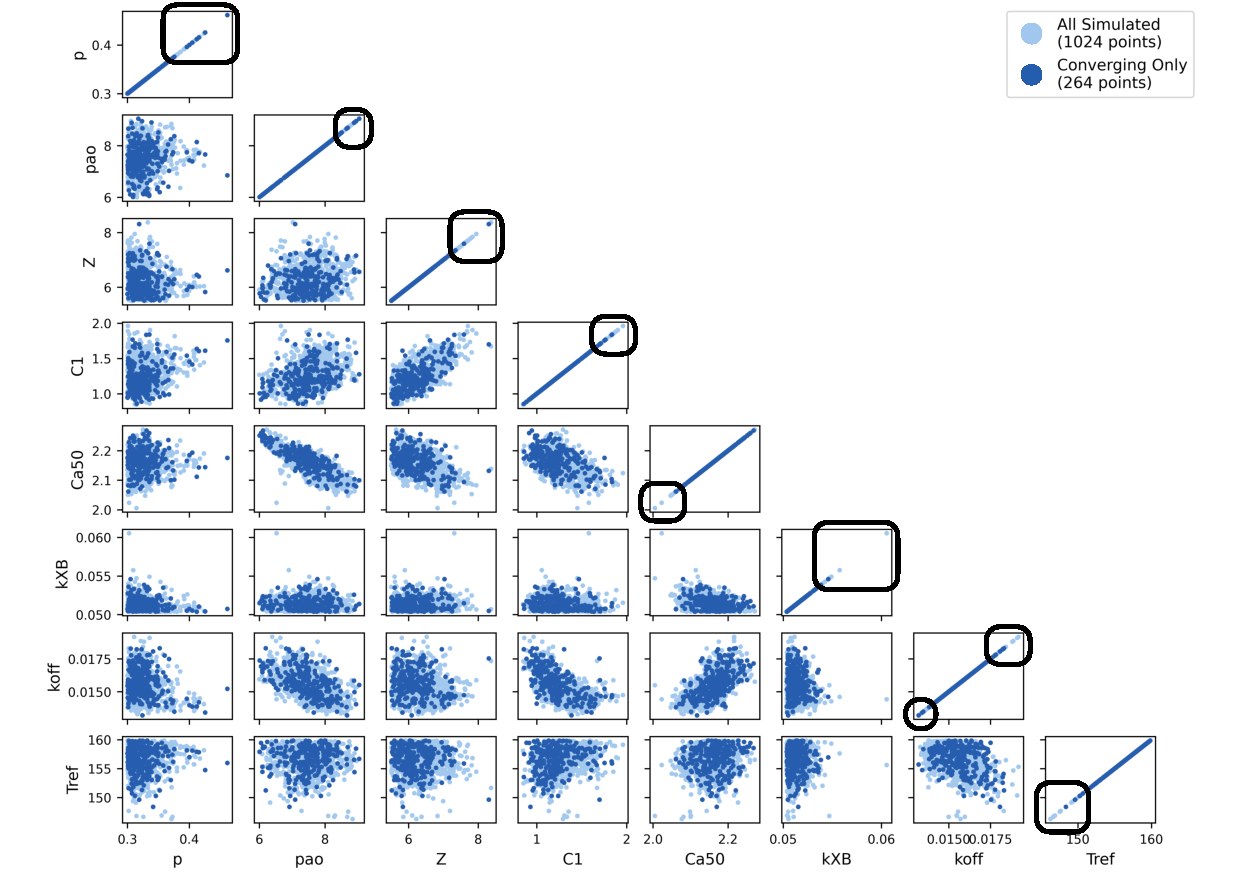
\includegraphics[width=\textwidth]{figures/chapter09/conv_vs_nonconv_sham.pdf}
    \caption{Non-implausible parameter space visual exploration for the SHAM rat model. The $8$D simulated input parameter space is plotted as a $2$D projection for each pair of parameters (light blue dots). The specific parameter sets leading to a converging mechanics simulation are further highlighted (dark blue dots) to spot regions of non-convergence. $1$D slices of the full space where a single parameter might have independently led to model failure are additionally marked with a black rectangular box.}
    \label{fig:shamnimpspaceexamined}
\end{figure}

\begin{figure}[ht!]
    \myfloatalign
    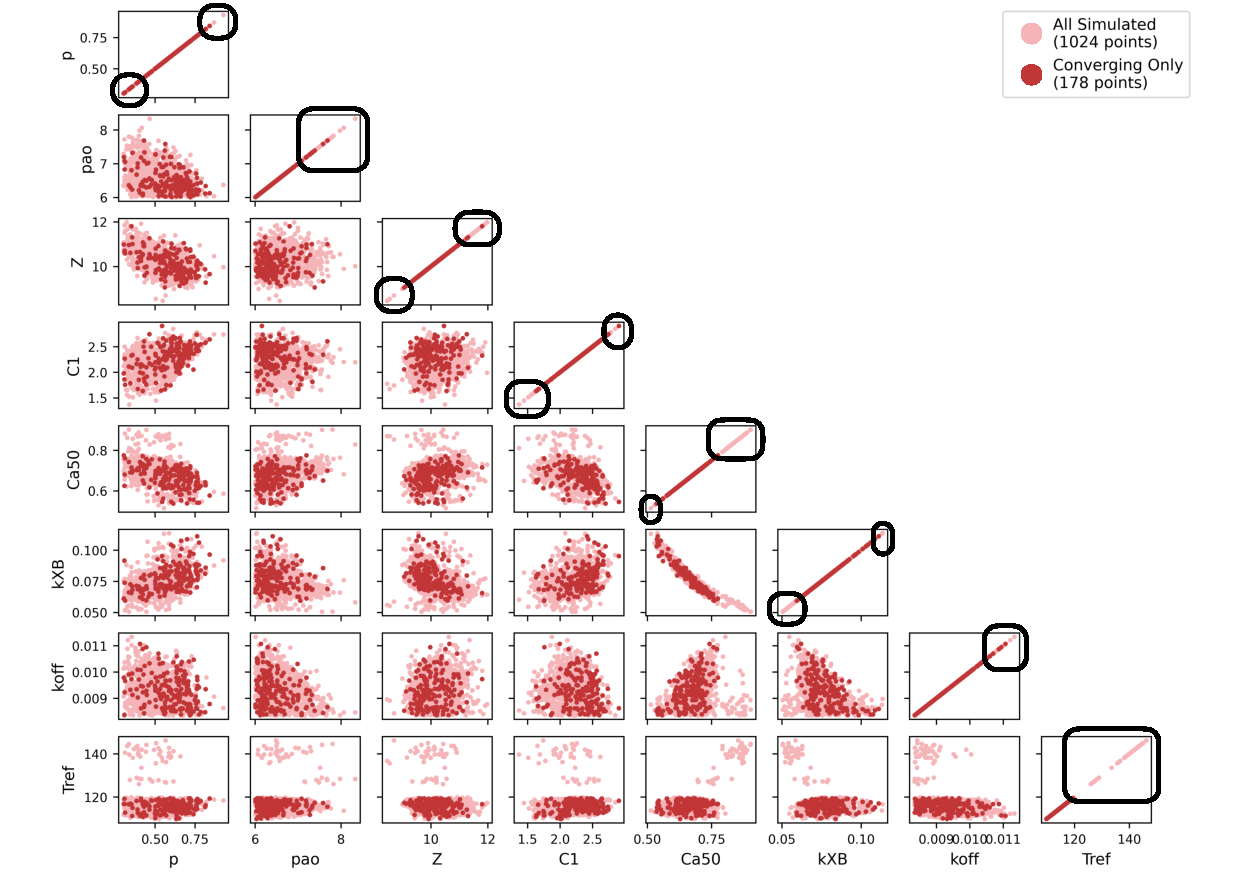
\includegraphics[width=\textwidth]{figures/chapter09/conv_vs_nonconv_ab.pdf}
    \caption{Non-implausible parameter space visual exploration for the AB rat model. The $8$D simulated input parameter space is plotted as a $2$D projection for each pair of parameters (light red dots). The specific parameter sets leading to a converging mechanics simulation are further highlighted (dark red dots) to spot regions of non-convergence. $1$D slices of the full space where a single parameter might have independently led to model failure are additionally marked with a black rectangular box.}
    \label{fig:abnimpspaceexamined}
\end{figure}

\vspace{0.2cm}
To conclude, it is worth mentioning that the developed rat heart contraction mechanics model is the combined result of different sub-modelling choices and assumptions, e.g. anatomy, fibre orientation, passive material properties, cell electrophysiology, tissue electrical activation, cell contraction, tissue contraction, spatial and haemodynamic boundary conditions (Chapter~\ref{cha:chapter02}). This means that the inferences become conditional on all of those assumptions being true, which could be a major source of discrepancy and therefore error in the final conclusions of any study we have presented within this thesis. Quantifying this discrepancy could go from looking for alternative modelling approaches i.e., different mathematical formulations for the same biological phenomena, through to simulating virtual populations of models.

%
%
%
\subsection{Experimental data}\label{sec:ch9experimental_data}
Throughout the entire thesis, we have made extensive use of experimental data from different sources. However, we were never able to obtain a consistent dataset of measurements coming from experiments all performed within the same laboratory and thus under the same conditions and following the same protocols.

\vspace{0.2cm}
For the first study, when fitting the healthy and diseased rat models (Chapter~\ref{cha:chapter4}), we had both the anatomy, cell electrophysiology and volumetric data coming from the same rat cohorts (SHAM and AB rats), although pressure data were taken from literature. In the second study for modelling the OM mechanisms of action (Chapter~\ref{cha:chapter5}), all the data used were collected from literature studies and for different species (rats for F-pCa data, pigs for LV haemodynamics data). For the third study, when performing model validation (Chapter~\ref{cha:chapter6}), we used literature data of very different rat heart preparations, which were examined under different experimental conditions, protocols and studies. Finally, in the fourth study for identifying possible pharmacological compounds' targets for treating rat HFpEF (Chapter~\ref{cha:chapter7}), we used ZSF1 rat data which came from many different literature studies.

\vspace{0.2cm}
The common strategy adopted in each of these studies was to project experimental observations into our current ``system space'' by means of averaging and percentages-of-variation calculation. Specifically, when the information about a specific feature value was provided in different studies, mean and standard deviation values for that feature were averaged to obtain the average mean and the average standard deviation for the feature across all the examined studies. This was a pragmatic choice; however, more formal approaches that make use of unbiased estimators of the sample mean and standard deviation could have been adopted to compute these statistics for a sample obtained as the combination of many samples, which also takes into account the dimension of each sample. Similarly, when the feature values could not be directly compared to our system values because the animal model was different or measurements were taken under different protocols, percentages of variation were first computed. These were then averaged as described above and finally applied to our system reference values.


%
%
%
\subsection{Model emulation, fitting and uncertainty quantification}\label{sec:ch9model_emulation_fitting_and_uncertainty_quantification}The use of emulators adds a layer of uncertainty in modelling the whole heart behaviour (LV contraction and relaxation). This is because emulators are probabilistic surrogates of the simulator, which is already an \textit{in silico} representation/approximation of the real world biological system. However, the speed-up that we gain by using emulators, which enables efficient model fitting and global sensitivity analysis, by far outweighs the loss in quantitative accuracy when making predictions. Unlike other supervised machine learning techniques used for regression such as nearest neighbours, linear/logistic regression, decision trees or neural networks, Gaussian process regression still relies on Bayesian statistics, providing confidence interval estimates on the predictions, which makes it the preferred choice to quantify uncertainty in the models.

\vspace{0.2cm}
For both HM and GSA, we used independent GPEs for each output. This univariate approach provided us with the flexibility to tune the hyperparameters and choose basis functions for each output independently. However, it did not account for potential correlations in outputs, which could be accounted for with a multivariate strategy (e.g.~\cite{Conti:2009}), although this assumes common hyperparameters across all outputs. The HM technique provides a bounded region of non-implausible parameter sets. Parameter bounds do not define parameter distributions. Including an MCMC parameter fit using the HM bounds as priors would extend this method to estimate likely parameter distributions as opposed to parameter bounds. In the used implausibility measure (equation~\eqref{eq:implmeasure}) calculation, we omitted the model discrepancy term (its variance was set to zero), for which we did not have any estimate available. However, to completely replace animal models with virtual representations of them, further experts knowledge will be needed to quantify the difference between the \textit{in silico} model and the real-world system that it represents.

\vspace{0.2cm}
Neglecting the model discrepancy was a pragmatic choice, mainly dictated by research time constraints, and we fully acknowledge the need for investing more energies towards a better characterisation of it, rather than mere neglect. In the context of HM, the poor representation (or, as in this case, no representation at all) of the model discrepancy can lead to biased and over-confident non-implausible input parameter values that cannot be used to generate trustworthy model predictions~\cite{Volodina:2021}. A first approach to address this issue would be to assign a weak prior information to the model discrepancy as initially proposed in~\cite{Kennedy:2001}. However, although this approach can be suitable for accurate interpolation, it could still not be enough to perform extrapolation or learn about physical model parameters, and a strong and meaningful prior information to specify the discrepancy distribution might be needed~\cite{Brynjarsdottir:2014}. There are formal ways of eliciting more realistic priors on the model discrepancy, and these in general aim at mathematically encoding modellers' knowledge about the underlying physical system in the form of constraints on prior distributions, as done in~\cite{Brynjarsdottir:2014} with constrains on a Gaussian process prior's derivatives. Other non-Bayesian approaches can be used, for example in~\cite{Wong:2017} a frequentist approach is employed to explicitly account for all potentially important sources of uncertainty including the structural one (model discrepancy). As computer simulators grow in complexity, their corresponding emulators introduce other sources of uncertainty, making the characterisation of model discrepancy nowadays still challenging.


%
%
%
\section{Next steps}\label{sec:ch9next_steps}
The next steps will go towards improving the methodology this thesis is heavily based on.

\vspace{0.2cm}
The first matter we want to address is the optimal collection of training dataset points via simulator evaluations. As more complex simulators will require more computational resources, or when predictions will have to be derived almost in real-time scenarios, we might not afford to simulate a whole parameter sweep (sampled with a space-filling design) anymore to construct the emulator training dataset. Space-filling designs assume that the samples provide information equally across the entire input space. Therefore, they perform exploration of the whole input space~\cite{Yue:2021}. However, these designs are not adaptive to the information from the response surface (input-output relationship). Identifying the nature of input-output relationships to subsequently choose design points one at a time is already possible through different \textit{acquisition functions} available in the literature for \textit{active learning} tasks (e.g.~\cite{Jones:1998,Pasolli:2011,Schreiter:2015}). For example, points can be selected such that they maximise an \textit{expected improvement} on a given objective function. This approach indeed realises a trade-off between exploration and exploitation. We aim to systematically incorporate an active learning component in our emulation framework to drastically reduce the number of simulator evaluations needed to build emulators for accurate regression.

\vspace{0.2cm}
The second topic of further investigation is the emulator structure we adopted. Specifically, we chose to use univariate emulators to map model input parameters to each of the LV scalar features independently. In future studies, we aim at investigating whether a multivariate approach can provide better model predictions. Building a multivariate GPE requires prescribing the covariance structure between the output components~\cite{Bonilla:2008,Rougier:2008,Conti:2010}, and it is not a trivial task. However, the output features we considered were extracted from two specific curves, namely the LVV and the LVP. This fact can be used to infer the correlations between output features belonging to the same curve. For example, in the case of the timing magnitudes ET, IVCT, IVRT, Tdiast we already know that their sum cannot exceed the cardiac cycle length. This information, along with other physiologically-derived arguments on LV volume and pressure transient morphologies, could be potentially used to prescribe the multivariate GPE covariance structure. Furthermore, a multivariate implausibility measure could be constructed from multivariate GPEs, and potentially assist in ruling out more implausible parameter space.

\vspace{0.2cm}
The third improvement we have in mind concerns the variance-based sensitivity analysis. We have seen that when using emulators to estimate the Sobol' sensitivity indices, the numerical error coming from having estimated expectations' and variances' integrals using quadrature formulae was not taken into account, but capturing the emulator uncertainty in the estimates was prioritised instead. In future work, we aim at quantifying how uncertainty in the emulator can propagate in the numerical error of the Sobol' indices calculation. We also aim at comparing Sobol' sensitivity analysis with other variance-based techniques where the underlying function is replaced by a surrogate model as in this case.


%
%
%
\section{Final remarks}\label{sec:ch9conclusions}
Calibrating complex multi-scale cardiac models to biological data, incorporating experimental measurements' uncertainty and propagating this forward into model predictions remains a challenge. However, these are all necessary features to incorporate if we want our virtual heart representation to be a reliable platform for testing hypotheses and aiding drug discovery and development. In this view, we have empathised the need for further research on better techniques towards a more synergic coupling between probabilistic tools and deterministic modelling. In this thesis, we have showcased this coupling in several applications, aligning with the currently increasing number of research outputs on this topic from the whole scientific community.